\makeatletter
\def\input@path{{../}}
\makeatother

\documentclass[/main.tex]{subfiles}
\graphicspath{{./pics/}{appAllResults/pics/}}
\begin{document}

\newcommand{\allmodeplots}[3]{% inputs are file name modifier, description of mode, and discription of gamma
  \FloatBarrier
  \begin{sidewaystable}[p]
    \caption[#3 of #2: Energy systematics table]{ \label{tab:energysystematics}
      Table of energy estimation uncertainties for the #3.
    }
    \resizebox{\textwidth}{!}{%
      \input{appAllResults/tables/table_#1_pseff.tex} }
  \end{sidewaystable}
  
  \begin{figure}[!htb]
    \centering
    \subfloat[Simulated BG Sum Energy Spectrum]{\includegraphics[width=.5\linewidth]{BGSumECuts_#1}}
    \subfloat[Simulated ES Sum Energy Spectrum]{\includegraphics[width=.5\linewidth]{ESSumECuts_#1}}\\
    \subfloat[Simulated BG Coincident Energy Spectrum]{\includegraphics[width=.5\linewidth]{BGCoinECuts_#1}}
    \subfloat[Simulated ES Coincident Energy Spectrum]{\includegraphics[width=.5\linewidth]{ESCoinECuts_#1}}
    \caption[#3 of #2: Sum and coincident simulated energy spectra with cuts]{
      Sum energy and coincident energy spectra for the #3.
    }
  \end{figure}
  
  \begin{figure}[p]
    \centering
    \subfloat[Simulation]{\includegraphics[width=0.7\linewidth]{BG2Dcuts_#1}}\\
    \subfloat[Data]{\includegraphics[width=0.7\linewidth]{Data2Dcuts_#1}}
    \caption[#3 of #2: 2D plots of sum and coincident energy cuts in simulations and data]{
      Simulated and measured multiplicity 2 energy spectrum with sum and coincident energy cuts included for the #3.
    }
  \end{figure}
  
  \begin{figure}[p]
    \centering
    \subfloat[Effect of all cuts on ROI]{\includegraphics[width=0.8\linewidth]{ESAllCuts_#1}}\\
    \subfloat[Table of efficiencies]{\input{appAllResults/tables/table_#1_efficiency.tex}}
    \caption[#3 of #2: Effect of all cuts in ROI]{Plot showing effect of cuts applied sequentially on ROI peak and table of detection efficiencies for the #3.}
  \end{figure}


  \begin{figure}[p]
    \centering
    \subfloat[Simulated BG Cuts]{\includegraphics[width=.5\linewidth]{BGAllCuts_#1}}
    \subfloat[Data Cuts]{\includegraphics[width=.5\linewidth]{DataAllCuts_#1}}\\
    \subfloat[Data ROIs]{\includegraphics[width=0.5\linewidth]{DataROIs_#1}}
    \caption[#3 of #2: Cuts appliled to simulated and measured background data]{
      Effect of all cuts applied to measured and simulated background data.
    }
  \end{figure}
  
  \begin{sidewaystable}[p]
    \centering
    \input{appAllResults/tables/table_#1_bgcuts.tex}
    \caption[#3 of #2: Summary of cut efficiency in BG and data]{
      Table of cut descriptions and efficiencies for simulated backgrounds and measured data for the #3.
    }
  \end{sidewaystable}
  \FloatBarrier
}

\onlyinsubfile{\appendix}
\chapter{Detailed Results for All Decay Modes}
\label{app:allresults}

The main document concerned itself primarily with the \tnbb\ of \Ge{76} to the \SP{0}{+}{1} excited state.
However, results are presented for all decay modes and energy peaks.
This appendix will present figures and tables detailing the simulations, cuts, efficiencies and results for each decay mode and peak.

\section{\tnbb\ to \SP{0}{+}{1}}
Note that both the 559~and 563~keV peaks will be shown together since they use the same sets of cuts.
\begin{figure}[!htb]
  \centering
  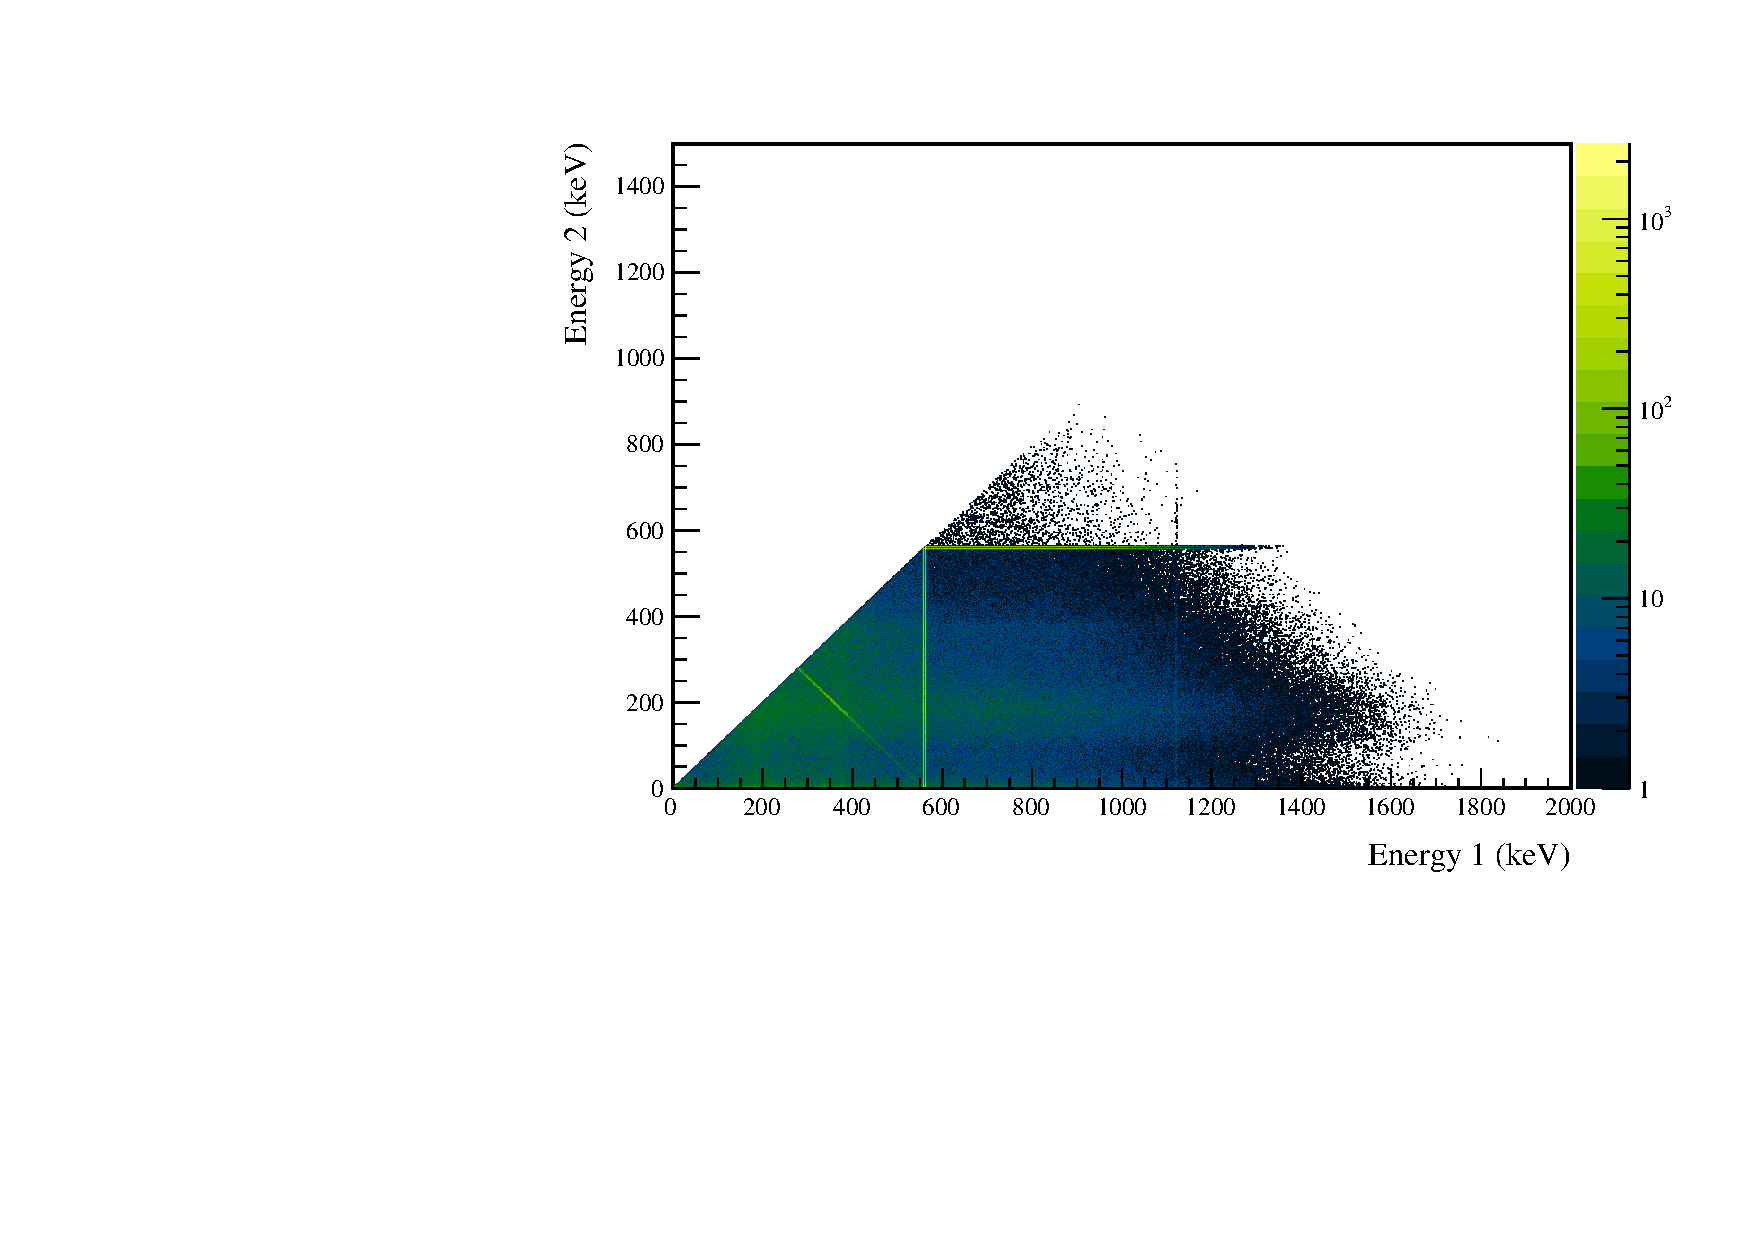
\includegraphics[width=.8\linewidth]{ESsim_2vBB_ES0_1}
  \caption[Simulation of \tnbb\ to \SP{0}{+}{1}]{
    Simulated multiplicity 2 energy spectrum of the \tnbb\ to \SP{0}{+}{1} decay mode}
\end{figure}

\allmodeplots{2vBB_ES0_1}{\tnbb\ to \SP{0}{+}{1}}{559~and 563~keV peaks}

\section{\tnbb\ to \SP{2}{+}{1}}
\begin{figure}[!htb]
  \centering
  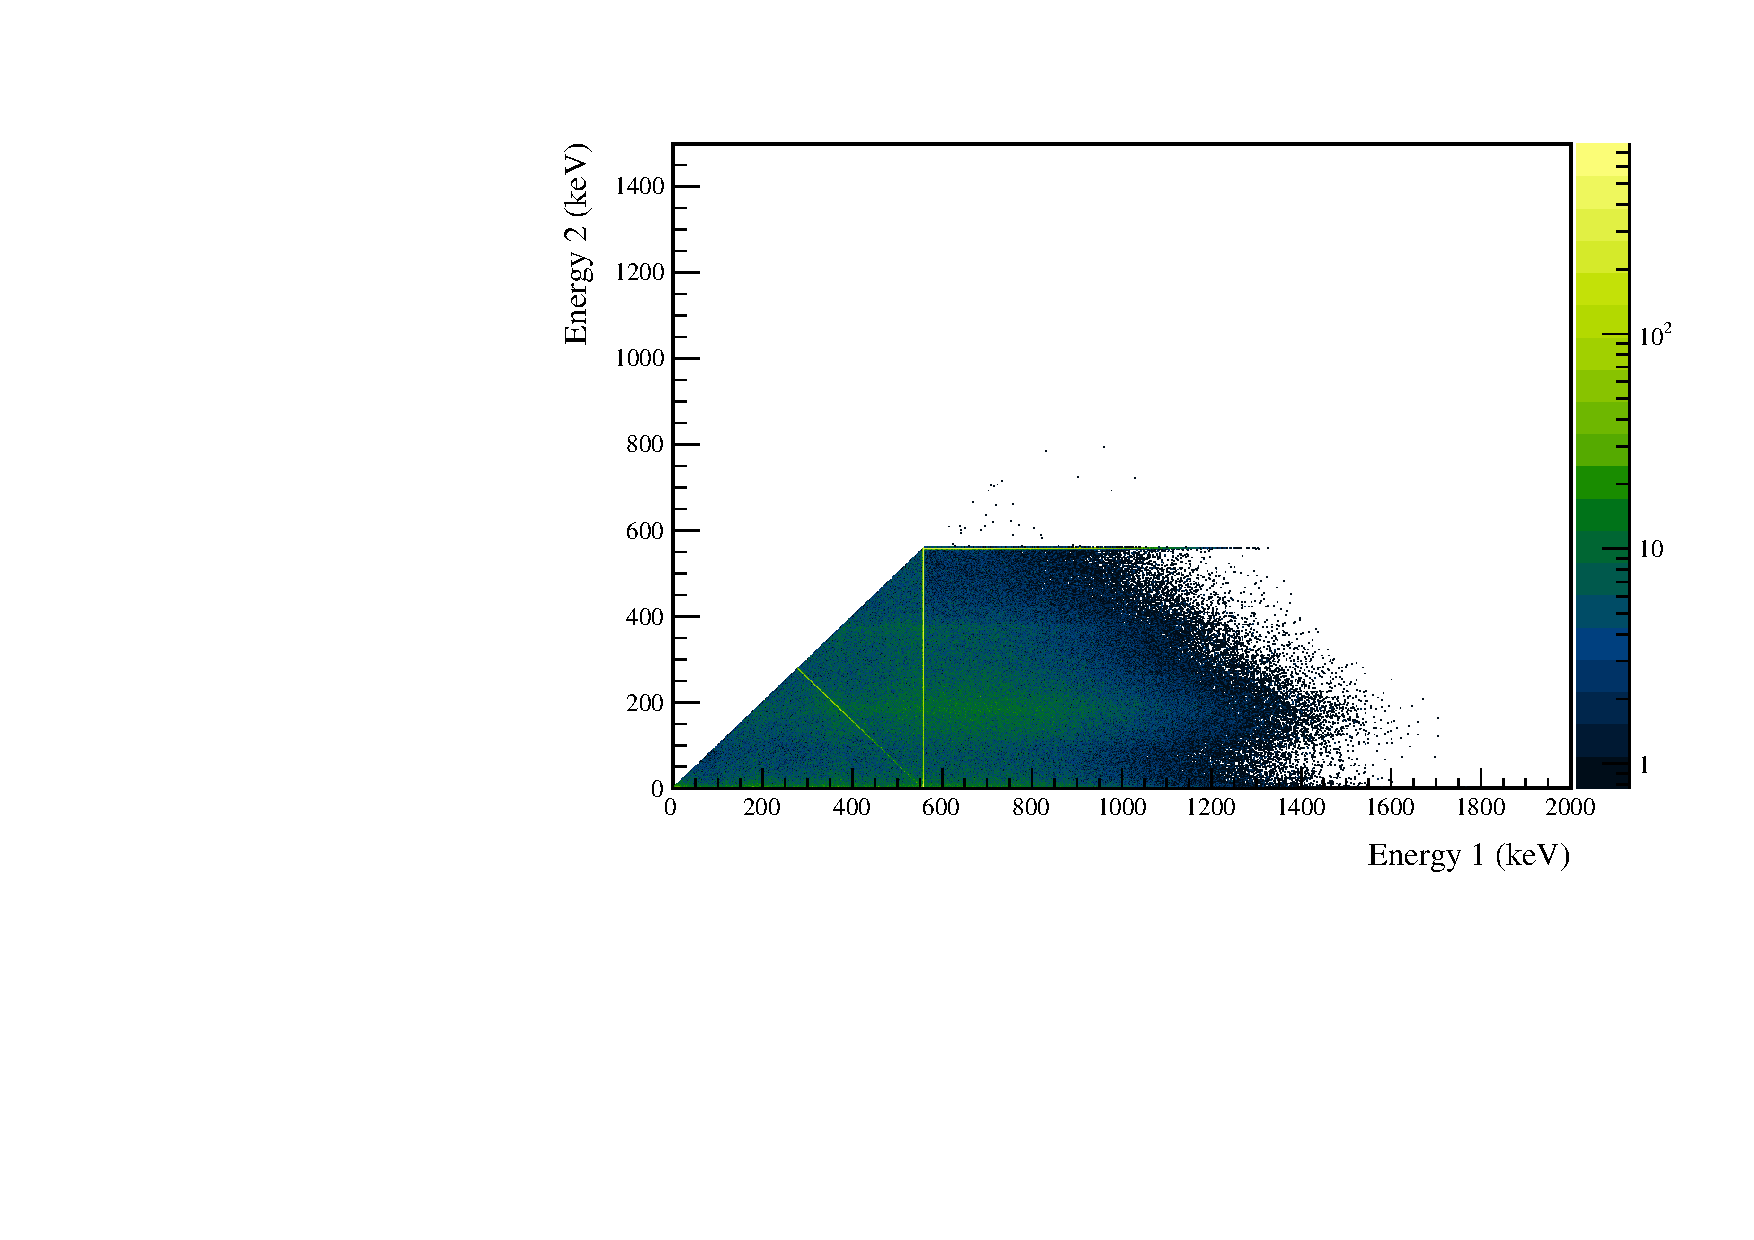
\includegraphics[width=.8\linewidth]{ESsim_2vBB_ES2_1}
  \caption[Simulation of \tnbb\ to \SP{2}{+}{1}]{
    Simulated multiplicity 2 energy spectrum of the \tnbb\ to \SP{2}{+}{1} decay mode}
\end{figure}

\allmodeplots{2vBB_ES2_1}{\tnbb\ to \SP{2}{+}{1}}{559~keV peak}

\section{\tnbb\ to \SP{2}{+}{2}}
\begin{figure}[!htb]
  \centering
  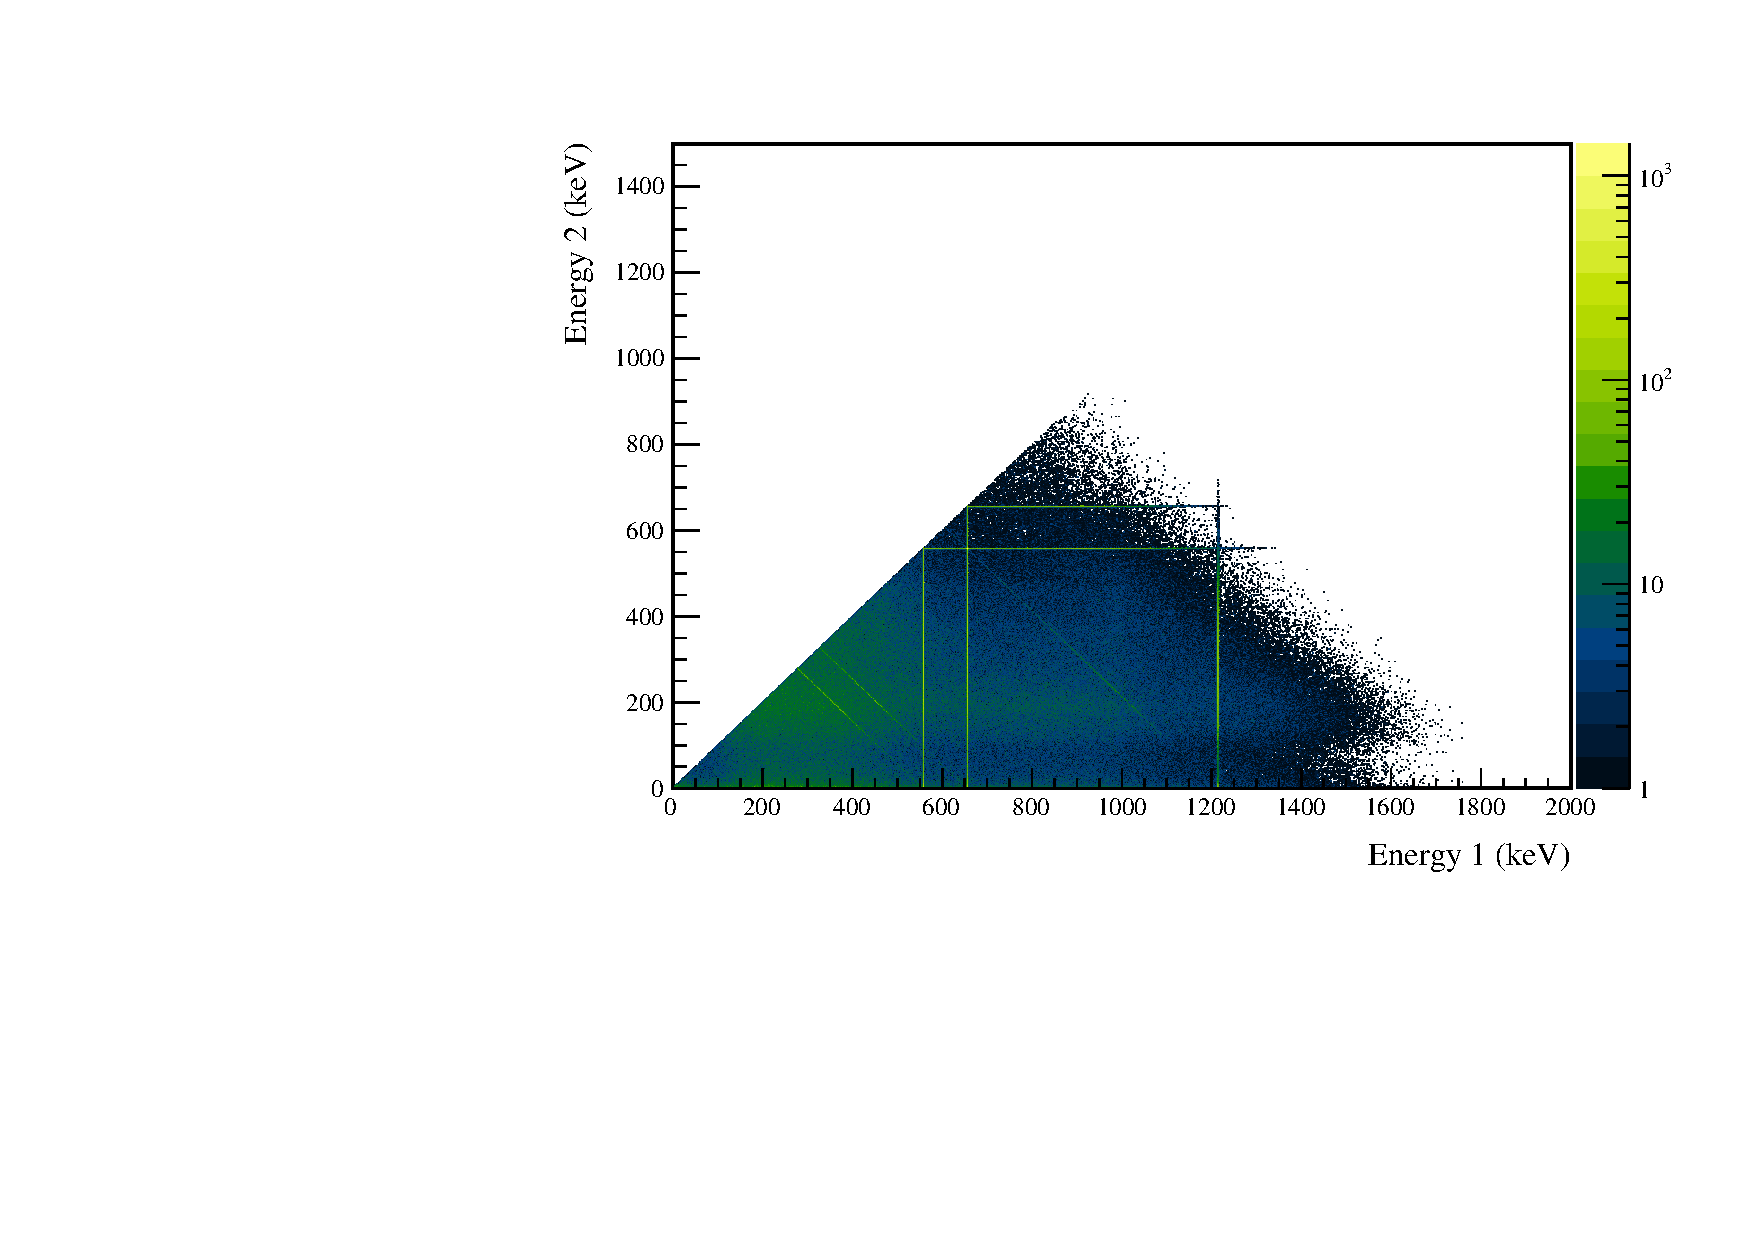
\includegraphics[width=.8\linewidth]{ESsim_2vBB_ES2_2}
  \caption[Simulation of \tnbb\ to \SP{2}{+}{2}]{
    Simulated multiplicity 2 energy spectrum of the \tnbb\ to \SP{2}{+}{2} decay mode}
\end{figure}

\subsection{559 keV peak}
\allmodeplots{2vBB_ES2_2_559}{\tnbb\ to \SP{2}{+}{2}}{559~keV peak}
\subsection{657 keV peak}
\allmodeplots{2vBB_ES2_2_657}{\tnbb\ to \SP{2}{+}{2}}{657~keV peak}
\subsection{1216 keV peak}
\allmodeplots{2vBB_ES2_2_1216}{\tnbb\ to \SP{2}{+}{2}}{1216~keV peak}



\section{\znbb\ to \SP{0}{+}{1}}
Note that both the 559~and 563~keV peaks will be shown together since they use the same sets of cuts.
\begin{figure}[!htb]
  \centering
  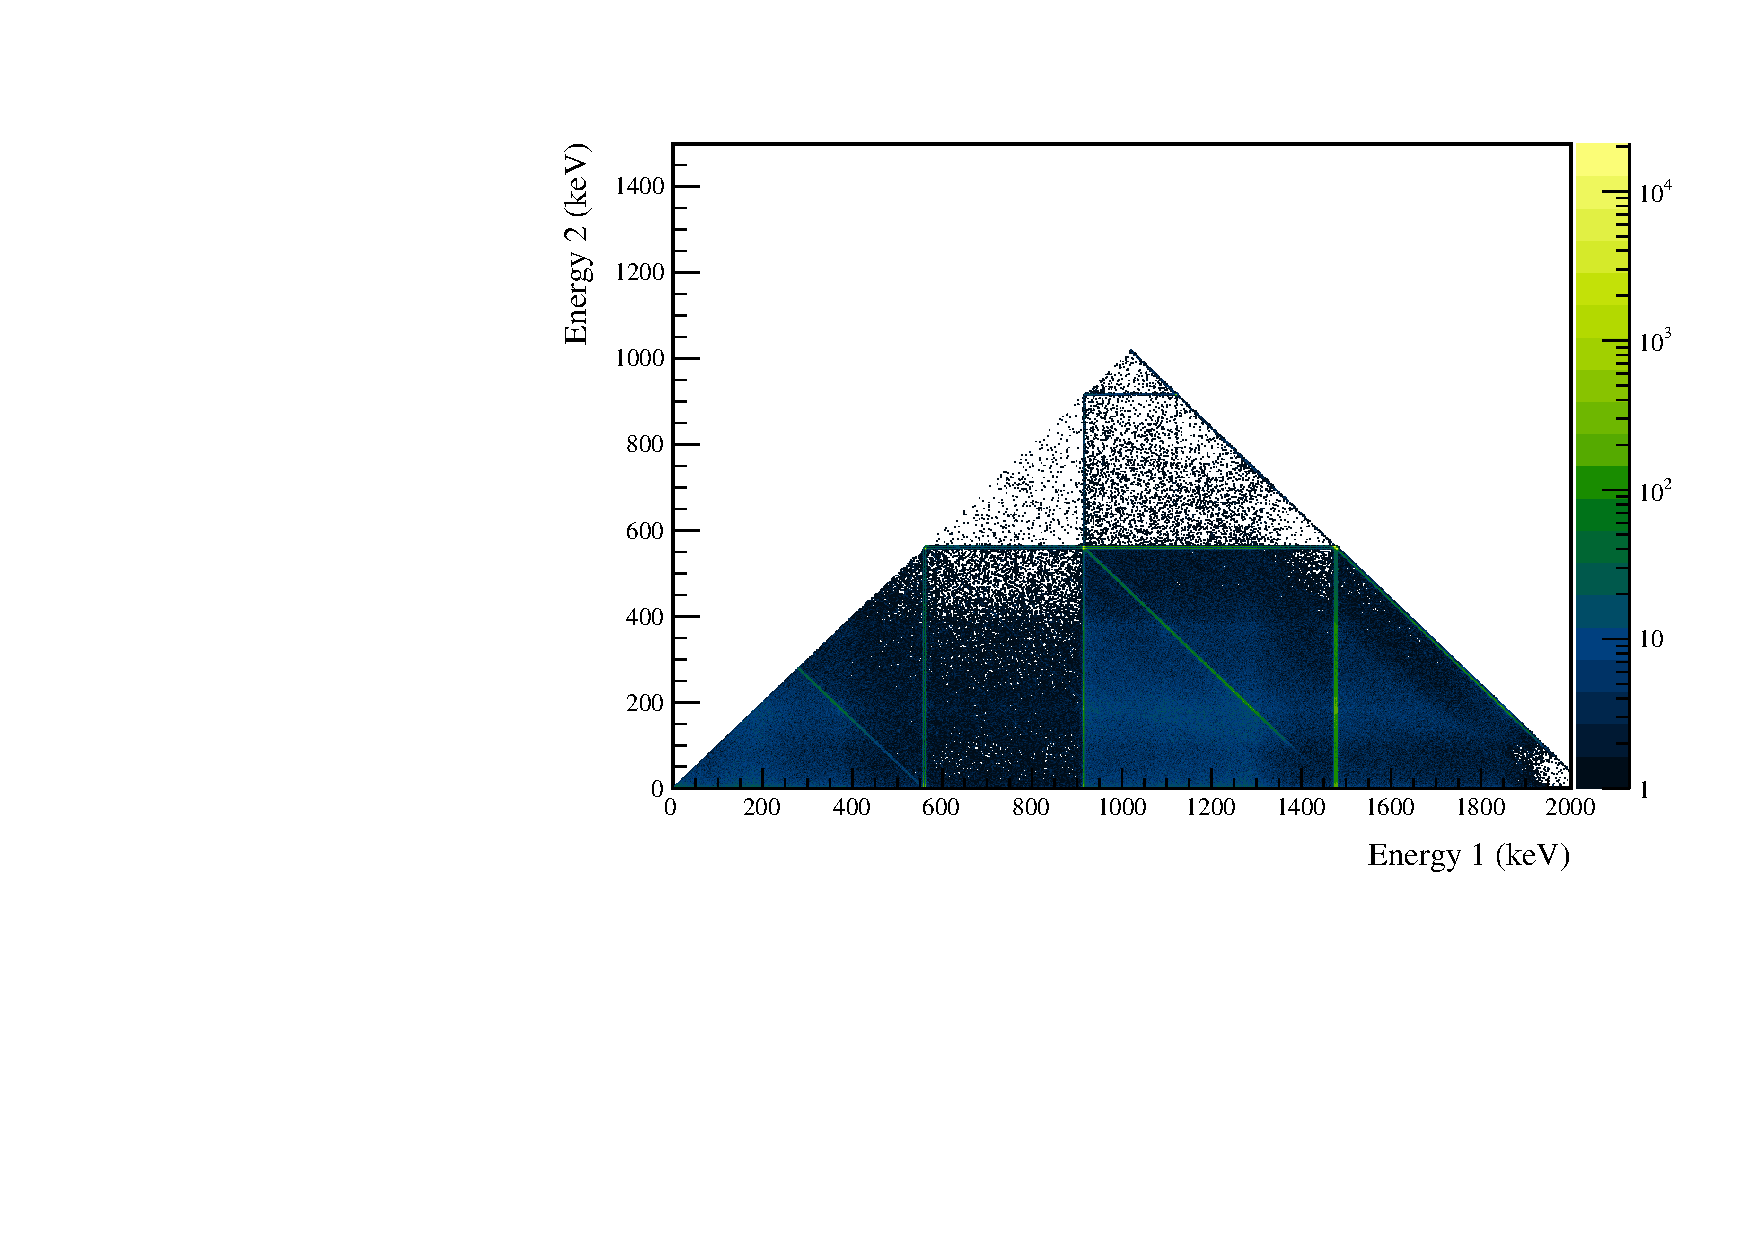
\includegraphics[width=.8\linewidth]{ESsim_0vBB_ES0_1}
  \caption[Simulation of \znbb\ to \SP{0}{+}{1}]{
    Simulated multiplicity 2 energy spectrum of the \znbb\ to \SP{0}{+}{1} decay mode}
\end{figure}

\allmodeplots{0vBB_ES0_1}{\znbb\ to \SP{0}{+}{1}}{559~and 563~keV peaks}

\section{\znbb\ to \SP{2}{+}{1}}
\begin{figure}[!htb]
  \centering
  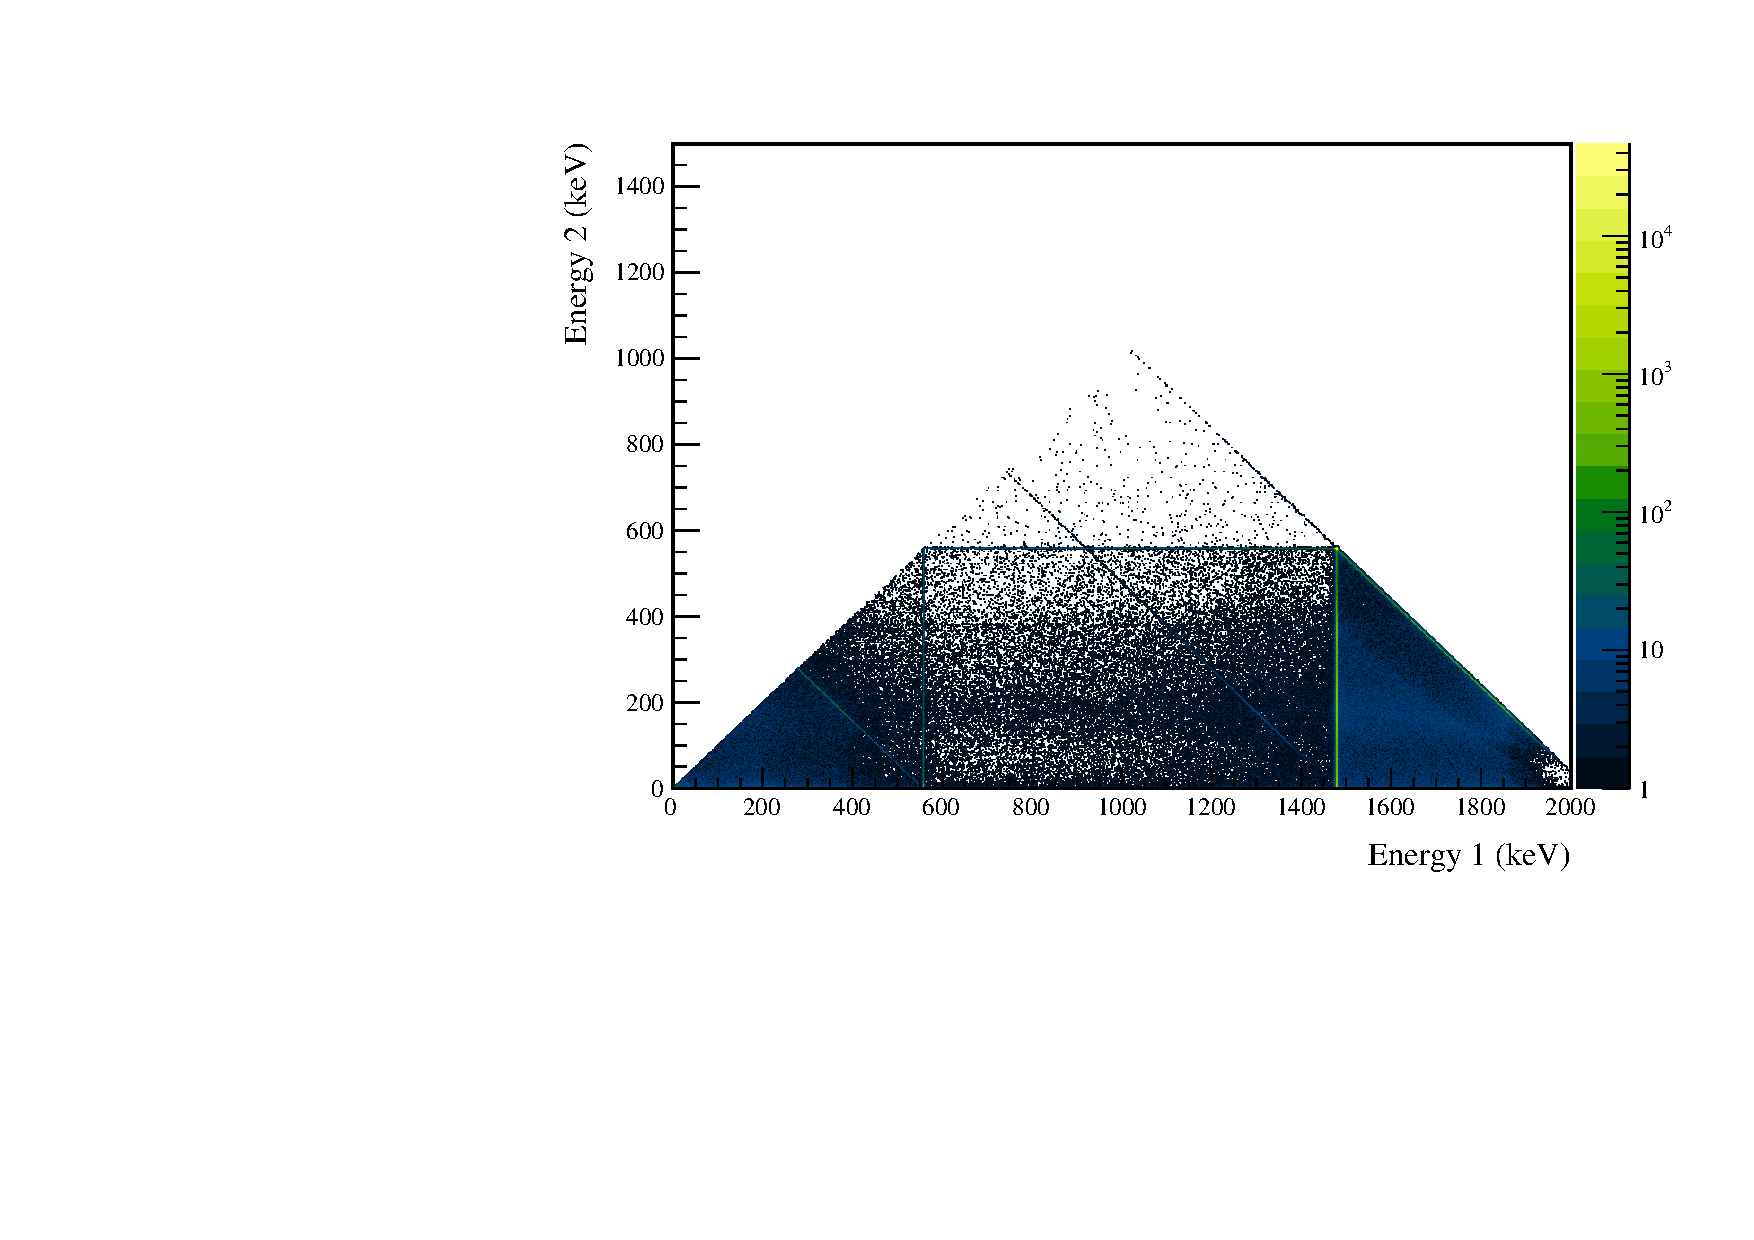
\includegraphics[width=.8\linewidth]{ESsim_0vBB_ES2_1}
  \caption[Simulation of \znbb\ to \SP{2}{+}{1}]{
    Simulated multiplicity 2 energy spectrum of the \znbb\ to \SP{2}{+}{1} decay mode}
\end{figure}

\allmodeplots{0vBB_ES2_1}{\znbb\ to \SP{2}{+}{1}}{559~keV peak}

\section{\znbb\ to \SP{2}{+}{2}}
\begin{figure}[!htb]
  \centering
  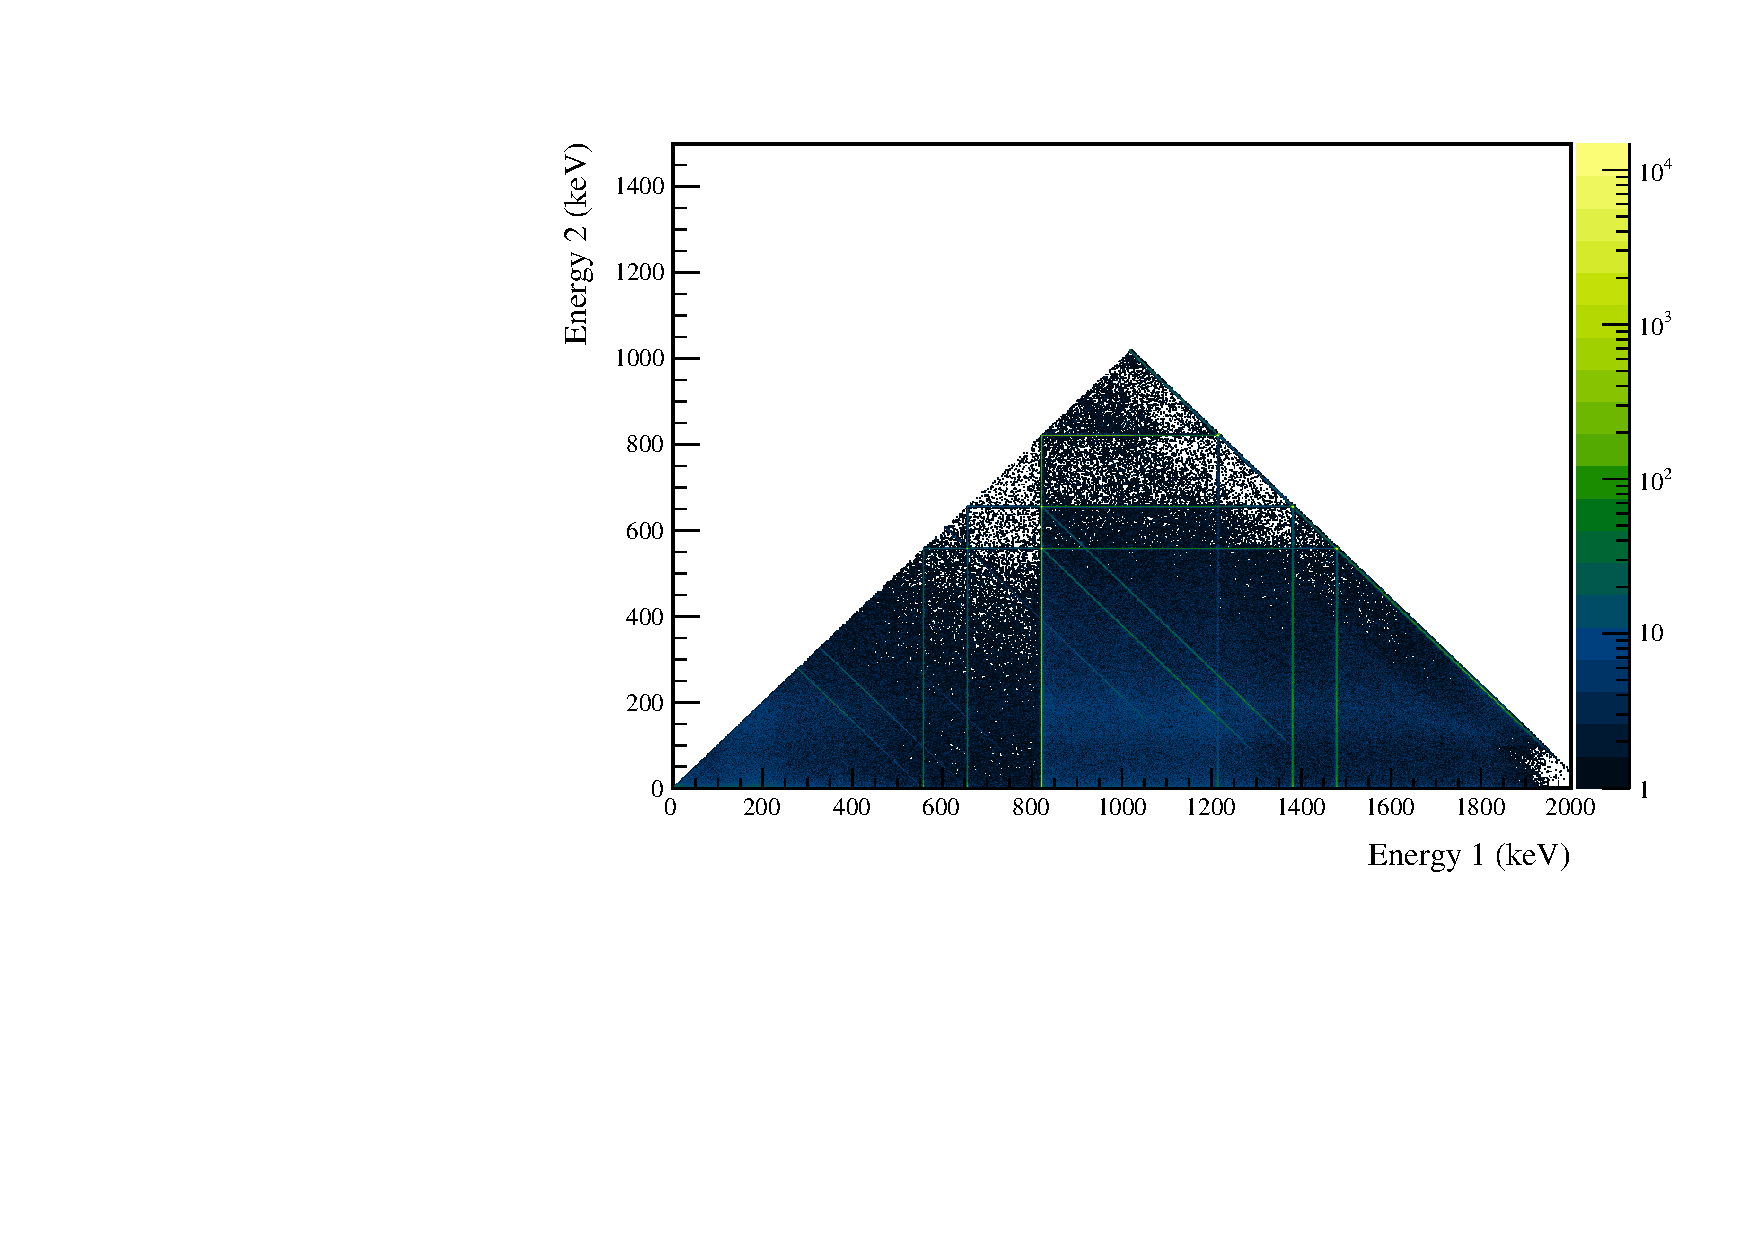
\includegraphics[width=.8\linewidth]{ESsim_0vBB_ES2_2}
  \caption[Simulation of \znbb\ to \SP{2}{+}{2}]{
    Simulated multiplicity 2 energy spectrum of the \znbb\ to \SP{2}{+}{2} decay mode}
\end{figure}

\subsection{559 keV peak}
\allmodeplots{0vBB_ES2_2_559}{\znbb\ to \SP{2}{+}{2}}{559~keV peak}
\subsection{657 keV peak}
\allmodeplots{0vBB_ES2_2_657}{\znbb\ to \SP{2}{+}{2}}{657~keV peak}
\subsection{1216 keV peak}
\allmodeplots{0vBB_ES2_2_1216}{\znbb\ to \SP{2}{+}{2}}{1216~keV peak}


\end{document}